\documentclass[12pt]{ociamthesis}
%%%%%%%%%%%%%%%%%%%%%%%%%%%%%%%%%%%%%%%%%% Disclaimer %%%%%%%%%%%%%%%%%%%%%%%%%%%%%%%%%%%%%%%%%%%%
% Based on the (unofficial) UPC thesis template:
%   https://github.com/sabirdvd/LaTeX-template-for-UPC-thesis-
% which is based on the Oxford thesis template:
%   https://github.com/mcmanigle/OxThesis
% Adapted for the SMDE first assignment (LaTeX version of the Typst report in ../report).
%%%%%%%%%%%%%%%%%%%%%%%%%%%%%%%%%%%%%%%%%% Disclaimer %%%%%%%%%%%%%%%%%%%%%%%%%%%%%%%%%%%%%%%%%%%%

% ---------- Encoding and language ----------
\usepackage[T1]{fontenc}
\usepackage[utf8]{inputenc}
\usepackage[english]{babel}

% ---------- Fonts ----------
\usepackage{palatino}               % main text (template font)
\usepackage[scaled=0.92]{helvet}    % sans serif, used on the title page

% ---------- Maths, graphics, colours ----------
\usepackage{amsmath,amssymb}
\usepackage{graphicx}
\usepackage{xcolor}
\graphicspath{{figures/}{images/}}  % charts written by the R scripts, and logos

% ---------- Tables and captions ----------
\usepackage{booktabs}               % \toprule, \midrule, \bottomrule
\usepackage{datatool}               % read the CSV tables written by the R scripts
\usepackage{caption}
\captionsetup{font=small, labelfont=bf}
\captionsetup[table]{skip=10pt}

% ---------- Lists ----------
\usepackage{enumitem}

% ---------- Sections: numbered 1, 1.1 (no chapters) ----------
\renewcommand{\thesection}{\arabic{section}}

% ---------- Header and footer ----------
\usepackage{fancyhdr}
\pagestyle{fancy}
\fancyhf{}
\renewcommand{\sectionmark}[1]{\markboth{\thesection\quad #1}{}}
\fancyhead[L]{\leftmark}
\fancyhead[R]{\thepage}

% ---------- Bibliography: numbered citations, refs.bib ----------
\usepackage[numbers]{natbib}
\bibliographystyle{plainnat}

% ---------- Links (load last) ----------
\usepackage{hyperref}
\usepackage{xurl}                   % long URLs (references) can break at any character
\definecolor{darkblue}{rgb}{0, 0, 0.5}
\hypersetup{
  colorlinks = true,
  urlcolor   = black,
  linkcolor  = red,
  citecolor  = darkblue,
  linktoc    = page,
}

% ---------- Report macros: \task, \csvtable, comments ----------
% ============================================================
% Report macros (LaTeX version of report/macros.typ)
% ============================================================

% ---------- Colours (same as report/settings.typ) ----------
\definecolor{upcblue}{HTML}{003B5C}
\definecolor{textgray}{HTML}{555555}
\definecolor{xfcolor}{HTML}{0066CC}
\definecolor{sscolor}{HTML}{008000}
\definecolor{aoccolor}{HTML}{8A2BE2}

\setlength{\emergencystretch}{2em}

% ---------- Comments ----------
% Show the author comments: set to \showtodofalse to hide them all
\newif\ifshowtodo
\showtodotrue

% \xfcomment{text}, \sscomment{text}, \aoccomment{text}
\newcommand{\authorcomment}[3]{\ifshowtodo{\par\noindent\raggedright\color{#1}\ttfamily\small #2: #3\par}\fi}
\newcommand{\xfcomment}[1]{\authorcomment{xfcolor}{XF}{#1}}
\newcommand{\sscomment}[1]{\authorcomment{sscolor}{SS}{#1}}
\newcommand{\aoccomment}[1]{\authorcomment{aoccolor}{AOC}{#1}}

% ---------- Question text under a subsection ----------
% \task{statement of the question}
\newcommand{\task}[1]{{\par\noindent\small\itshape\color{textgray}#1\par}\medskip}

% ---------- Table from a CSV file written by the R scripts ----------
% \csvtable[size]{name}{caption}{label}
%   size:    optional font size of the table (default \small)
%   name:    file name without extension (q1b_summary -> tables/q1b_summary.csv)
%   caption: caption above the table (numbered "Table N")
%   label:   label to reference it with \autoref{label}, e.g. tab:q1b-summary
% The first CSV row is the header; columns with numbers are right-aligned,
% the others left-aligned (datatool detects the type of each column).
\renewcommand{\dtldisplaystarttab}{\toprule}
\renewcommand{\dtldisplayafterhead}{\midrule}
\renewcommand{\dtldisplayendtab}{\\\bottomrule}
\newcommand{\csvtable}[4][\small]{%
  \DTLifdbexists{#2}{}{\DTLloadrawdb{#2}{tables/#2.csv}}%
  \begin{table}[htbp]
    \centering
    #1
    \caption{#3}\label{#4}
    \DTLdisplaydb{#2}
  \end{table}%
}

% ---------- References ----------
\renewcommand{\bibsection}{\section*{References}\addcontentsline{toc}{section}{References}\markboth{References}{}}

% ---------- Appendix ----------
% Sections after \startappendix are numbered A, B, ... on a new page
\newcommand{\startappendix}{%
  \clearpage
  \setcounter{section}{0}
  \renewcommand{\thesection}{\Alph{section}}%
}


% ---------- Title page (see \maketitle in ociamthesis.cls) ----------
\title{First Assignment}
\author{Simin S. \\ Antonina Oliwia C. \\ Xiang Feng Y.}
\course{Statistical Modelling and Design of Experiments (SMDE) \\ Fall 2026}
\degree{Master in Innovation and Research in Informatics (MIRI)}
\doctype{Assignment report}
\faculty{Facultat d'Informàtica de Barcelona (FIB)}
\university{Universitat Politècnica de Catalunya (UPC) -- BarcelonaTech}
\titlelogo{logo-upc-fib}

\begin{document}

% line spacing of the template
\baselineskip=18pt plus1pt

\setcounter{secnumdepth}{3}
\setcounter{tocdepth}{2}

\maketitle

\begin{romanpages}          % roman page numbers for the contents
\tableofcontents
\end{romanpages}            % the body is numbered from page 1 (12-page limit without the appendix)

% ============================================================
% 1. FIRST QUESTION
% ============================================================
\section{Visualisation, Chi-Square and t-Test}\label{sec:q1}

% ------------------------------------------------------------
% a)
% ------------------------------------------------------------
\subsection{Data Import and Variable Types}\label{sec:q1a}

\task{Import the data set to R assigning the type of each variable correctly.}

We imported the data set \texttt{bodyPerformance.csv} and renamed its columns to short R names without spaces or symbols (e.g.\ \texttt{body fat\_\%} becomes \texttt{body\_fat\_pct}).

Then we gave each variable the type that matches its measurement scale:

\begin{itemize}
  \item \textbf{Nominal categorical:} \texttt{gender} is a factor, and we labeled its codes \texttt{F} and \texttt{M} as \texttt{Female} and \texttt{Male} respectively.
  \item \textbf{Ordinal categorical:} \texttt{class} is an ordered factor with the levels $D < C < B < A$, from poor to excellent performance.
  \item \textbf{Numerical:} the other ten variables (\texttt{age}, \texttt{height\_cm}, \texttt{weight\_kg}, \texttt{body\_fat\_pct}, \texttt{diastolic}, \texttt{systolic}, \texttt{grip\_force}, \texttt{sit\_bend\_cm}, \texttt{sit\_ups} and \texttt{broad\_jump\_cm}) are numeric.
    \texttt{age} could be stored as an integer, but we kept it numeric for simplicity.
\end{itemize}

The result has 13,393 observations of 12 variables with no missing values (R output, Appendix~\ref{app:code}).
The name, type and levels of each variable are listed in \autoref{tab:q1a-variables}.

% ------------------------------------------------------------
% b)
% ------------------------------------------------------------
\subsection{Descriptive Statistics}\label{sec:q1b}

\task{Summarize the numerical variables and analyze their distributions.}

\paragraph{Outliers.} \autoref{tab:q1b-summary} summarizes the ten numerical variables of the original data set, and their boxplots (\autoref{fig:q1b-boxplots}) show values beyond $1.5 \times \mathrm{IQR}$ from the quartiles in every variable except \texttt{age} and \texttt{sit\_ups} (\autoref{tab:q1b-outliers}).
Most of these outliers are possible values, so instead of removing all of them we compared the extreme values of \autoref{tab:q1b-summary} with the adult health reference ranges of \autoref{tab:q1b-reference}, and removed only the observations with impossible values (\autoref{tab:q1b-removed}):

\begin{itemize}
  \item \textbf{Blood pressure:} the readings with \texttt{systolic} $< 70$ or \texttt{diastolic} $< 40$\,mmHg (e.g.\ 0/0, 14/67 and 145/6), far below the hypotension limit of 90/60\,mmHg \citep{nhs_hypotension}, and those with \texttt{systolic} $\leq$ \texttt{diastolic} (e.g.\ 104/156.2 and 95/99), since the systolic pressure is by definition the higher of the two.
  \item \textbf{Body fat:} the values below the essential fat, which is 2--5\% for men and 10--13\% for women (3.5, 9.4 and 9.7\% in women), and the maximum of 78.4\%, far above the obesity limit of 25\% for men and 32\% for women \citep{ace_bodyfat}.
  \item \textbf{Performance tests:} the zeros of \texttt{grip\_force} and \texttt{broad\_jump\_cm}, which mean that the test was not done rather than a measurement, and the two maxima of \texttt{sit\_bend\_cm} (185 and 213\,cm), far from the rest of its values (at most 42\,cm).
\end{itemize}

In total we removed 28 observations (0.2\%) and saved the other 13,365 as \texttt{bodyPerformance\_clean.csv}, the data set used in the rest of the assignment (Sections~\ref{sec:q1c}--\ref{sec:q1g} and \ref{sec:q2}).
We kept the other outliers because they are possible values: the high blood pressures correspond to stage~2 hypertension or a hypertensive crisis (up to 201\,mmHg) \citep{whelton2018}, the 3\% body fat of some men is within their essential fat \citep{ace_bodyfat}, the shortest and lightest individuals have a BMI of severe thinness ($< 16$) \citep{who1995}, which is rare but possible, and the 125 zeros of \texttt{sit\_ups} correspond to individuals who could not do any sit-up.

\paragraph{Distribution and normality.}
\xfcomment{TODO: describe the shape of each variable with the histograms of the cleaned data (\autoref{fig:q1b-histograms}) and compare it with the mean and median of \autoref{tab:q1b-summary}.}
\xfcomment{TODO: check whether the two peaks of \texttt{grip\_force} (around 25 and 43) correspond to the two values of \texttt{gender} (Section~\ref{sec:q1g}).}
\xfcomment{TODO: comment on the Q-Q plots of the cleaned data (\autoref{fig:q1b-qqplots}): which variables follow the line and which deviate in the tails.}
\xfcomment{TODO: report the Shapiro-Wilk test on a random sample of 5,000 cleaned observations (\autoref{tab:q1b-shapiro}) and explain why, with this sample size, it rejects normality even for the variables that look normal in \autoref{fig:q1b-histograms}.}

% ------------------------------------------------------------
% c)
% ------------------------------------------------------------
\subsection{Blood Pressure by Gender}\label{sec:q1c}

\task{Consider the variables of diastolic and systolic blood pressure.
Eliminate the zero values and check their distributions for the gender groups using proper graph(s).
Interpret your findings.}

\xfcomment{Discuss the differences in the distributions of \texttt{diastolic} and \texttt{systolic} between the two levels of \texttt{gender}, based on your graphs.}

% ------------------------------------------------------------
% d)
% ------------------------------------------------------------
\subsection{Confidence Intervals for Systolic Blood Pressure}\label{sec:q1d}

\task{Construct 95\% confidence intervals for the mean systolic blood pressure of two gender groups and interpret them.}

\xfcomment{State the resulting intervals and explain their practical meaning in context.}

% ------------------------------------------------------------
% e)
% ------------------------------------------------------------
\subsection{Age Groups}\label{sec:q1e}

\task{Categorize the variable age into four categories cutting from the values 30, 40 and 50 and save it as a new variable into your data frame.}

We saved the four age groups as the new variable \texttt{age\_cat}; their frequencies are in \autoref{tab:q1e-age-groups} and \autoref{fig:q1e-age-groups}.

\xfcomment{TODO: comment on the size of each level of \texttt{age\_cat} (e.g.\ the largest and smallest groups).}

% ------------------------------------------------------------
% f)
% ------------------------------------------------------------
\subsection{Association of Age Groups with Class and Gender}\label{sec:q1f}

\task{Analyze the association first between age groups and class and then between age groups and gender by using proper statistical method.}

The contingency tables are in \autoref{tab:q1f-age-class} and \autoref{tab:q1f-age-gender}, the chi-square tests of independence in \autoref{tab:q1f-chisq} and the proportions of each level of \texttt{class} and \texttt{gender} within each level of \texttt{age\_cat} in \autoref{fig:q1f-proportions}.

\xfcomment{TODO: state the hypotheses, check the assumption (expected counts $\geq 5$), report $\chi^2$, df and p-value, and conclude on the independence of \texttt{age\_cat} with \texttt{class} and with \texttt{gender}.}

% ------------------------------------------------------------
% g)
% ------------------------------------------------------------
\subsection{Physical Performance by Gender}\label{sec:q1g}

\task{Test whether physical performance test results of the individuals are affected from the gender.
Check the assumptions and visualize the relationship between these two characteristics.}

\xfcomment{Summarize the assumption checks and discuss whether \texttt{grip\_force}, \texttt{sit\_bend\_cm}, \texttt{sit\_ups} and \texttt{broad\_jump\_cm} differ significantly by \texttt{gender}.}

% ============================================================
% 2. SECOND QUESTION
% ============================================================
\section{Title of Question 2}\label{sec:q2}

\subsection{Title of Part a}\label{sec:q2a}

\task{Statement of part a.}

\xfcomment{Your analysis here.}

\subsection{Title of Part b}\label{sec:q2b}

\task{Statement of part b.}

\xfcomment{Your analysis here.}

% ============================================================
% 3. THIRD QUESTION
% ============================================================
\section{Title of Question 3}\label{sec:q3}

\subsection{Title of Part a}\label{sec:q3a}

\task{Statement of part a.}

\xfcomment{Your analysis here.}

\subsection{Title of Part b}\label{sec:q3b}

\task{Statement of part b.}

\xfcomment{Your analysis here.}


% ---------- Appendix: sections A, B, ... ----------
\startappendix
% ============================================================
% APPENDIX A: TABLES (CSV files written by R/Q*.R in tables/)
% ============================================================
\section{Tables}\label{app:tables}

\subsection{Question 1}

\csvtable{q1a_variables}
  {Variables of the data set: name in R, original name, type and levels.}
  {tab:q1a-variables}

\csvtable{q1b_summary}
  {Summary statistics of the numerical variables (original data).}
  {tab:q1b-summary}

\csvtable{q1b_outliers}
  {Number of outliers ($1.5 \times \mathrm{IQR}$ rule) and of zero values of the numerical variables.}
  {tab:q1b-outliers}

\csvtable[\footnotesize]{q1b_removed}
  {Observations removed as impossible values: rule, removed values (\texttt{systolic}/\texttt{diastolic} for blood pressure) and number of rows.}
  {tab:q1b-removed}

\begin{table}[htbp]
  \centering
  \footnotesize
  \caption{Reference ranges of the health measures for adults. Sources: BMI \citep{who1995, who2000}, \texttt{body\_fat\_pct} \citep{ace_bodyfat}, \texttt{systolic} and \texttt{diastolic} \citep{nhs_hypotension, whelton2018} and \texttt{grip\_force} \citep{dodds2014}.}
  \label{tab:q1b-reference}
  \begin{tabular}{lll}
    \toprule
    Measure & Category & Range \\
    \midrule
    BMI (kg/m$^2$), from
      & Severe thinness       & $< 16$ \\
    \quad \texttt{height\_cm}, \texttt{weight\_kg}
      & Underweight           & $< 18.5$ \\
      & Normal weight         & 18.5--24.9 \\
      & Overweight            & 25--29.9 \\
      & Obesity               & $\geq 30$ \\
    \midrule
    \texttt{body\_fat\_pct} (\%),
      & Essential fat         & 2--5 / 10--13 \\
    \quad men / women
      & Athletes              & 6--13 / 14--20 \\
      & Fitness               & 14--17 / 21--24 \\
      & Average               & 18--24 / 25--31 \\
      & Obesity               & $\geq 25$ / $\geq 32$ \\
    \midrule
    \texttt{systolic} / \texttt{diastolic}
      & Low (hypotension)     & $< 90$ / $< 60$ \\
    \quad (mmHg)
      & Normal                & $< 120$ and $< 80$ \\
      & Elevated              & 120--129 and $< 80$ \\
      & Stage 1 hypertension  & 130--139 or 80--89 \\
      & Stage 2 hypertension  & $\geq 140$ or $\geq 90$ \\
      & Hypertensive crisis   & $> 180$ and/or $> 120$ \\
    \midrule
    \texttt{grip\_force} (kg),
      & Peak median (ages 26--42) & 51 / 31 \\
    \quad men / women & & \\
    \bottomrule
  \end{tabular}
\end{table}

\csvtable{q1b_shapiro}
  {Shapiro-Wilk p-value of the numerical variables (random sample of 5,000 observations of the cleaned data).}
  {tab:q1b-shapiro}
\csvtable{q1e_age_groups}
  {Frequency of each age group (\texttt{age\_cat}).}
  {tab:q1e-age-groups}

\csvtable{q1f_age_class}
  {Contingency table of age group and performance class.}
  {tab:q1f-age-class}

\csvtable{q1f_age_gender}
  {Contingency table of age group and gender.}
  {tab:q1f-age-gender}

\csvtable{q1f_chisq}
  {Chi-square tests of independence: statistic, degrees of freedom, p-value and smallest expected count.}
  {tab:q1f-chisq}

% ============================================================
% APPENDIX B: FIGURES (PNG files written by R/Q*.R in figures/)
% ============================================================
\clearpage
\section{Figures}\label{app:figures}

\subsection{Question 1}

\begin{figure}[htbp]
  \centering
  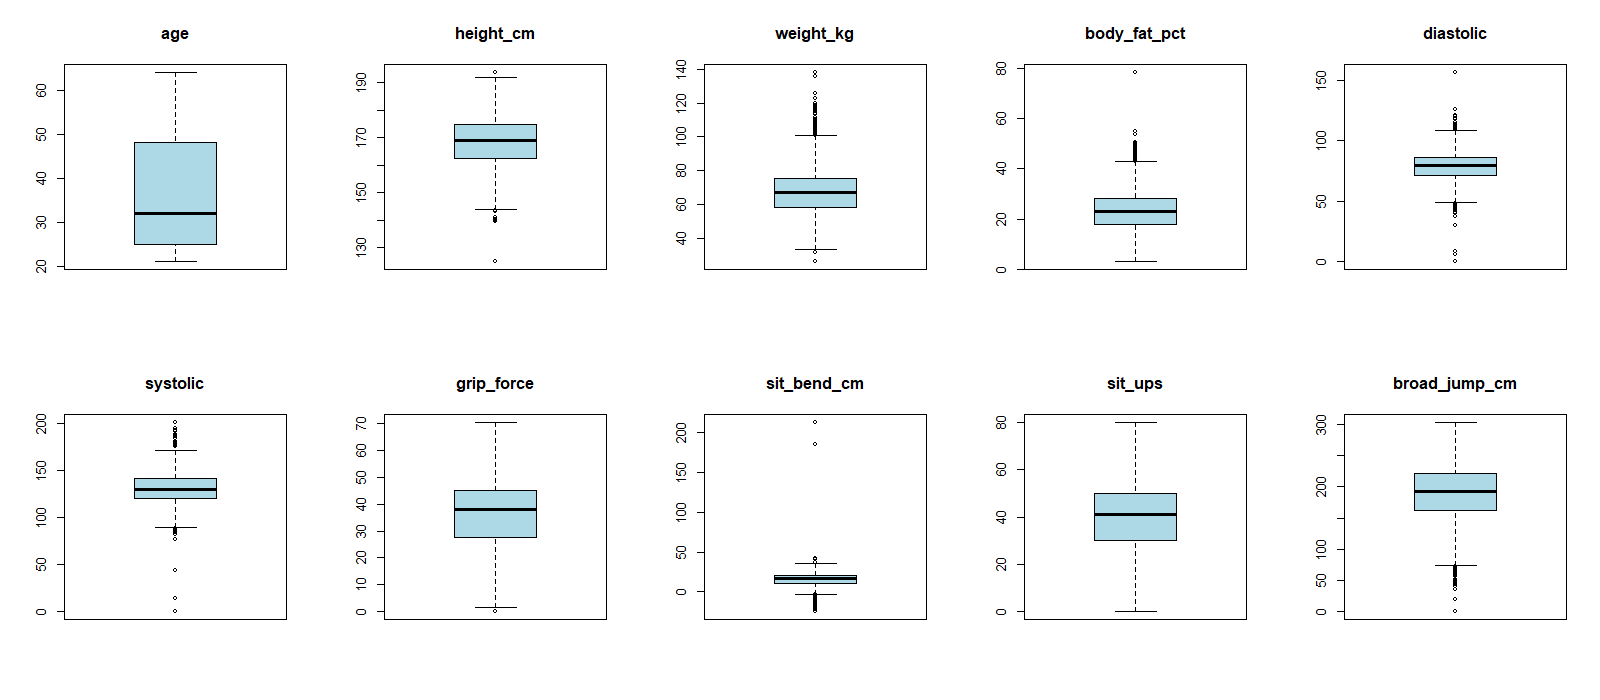
\includegraphics[width=\linewidth]{q1b_boxplots}
  \caption{Boxplots of the numerical variables (original data).}
  \label{fig:q1b-boxplots}
\end{figure}

\begin{figure}[htbp]
  \centering
  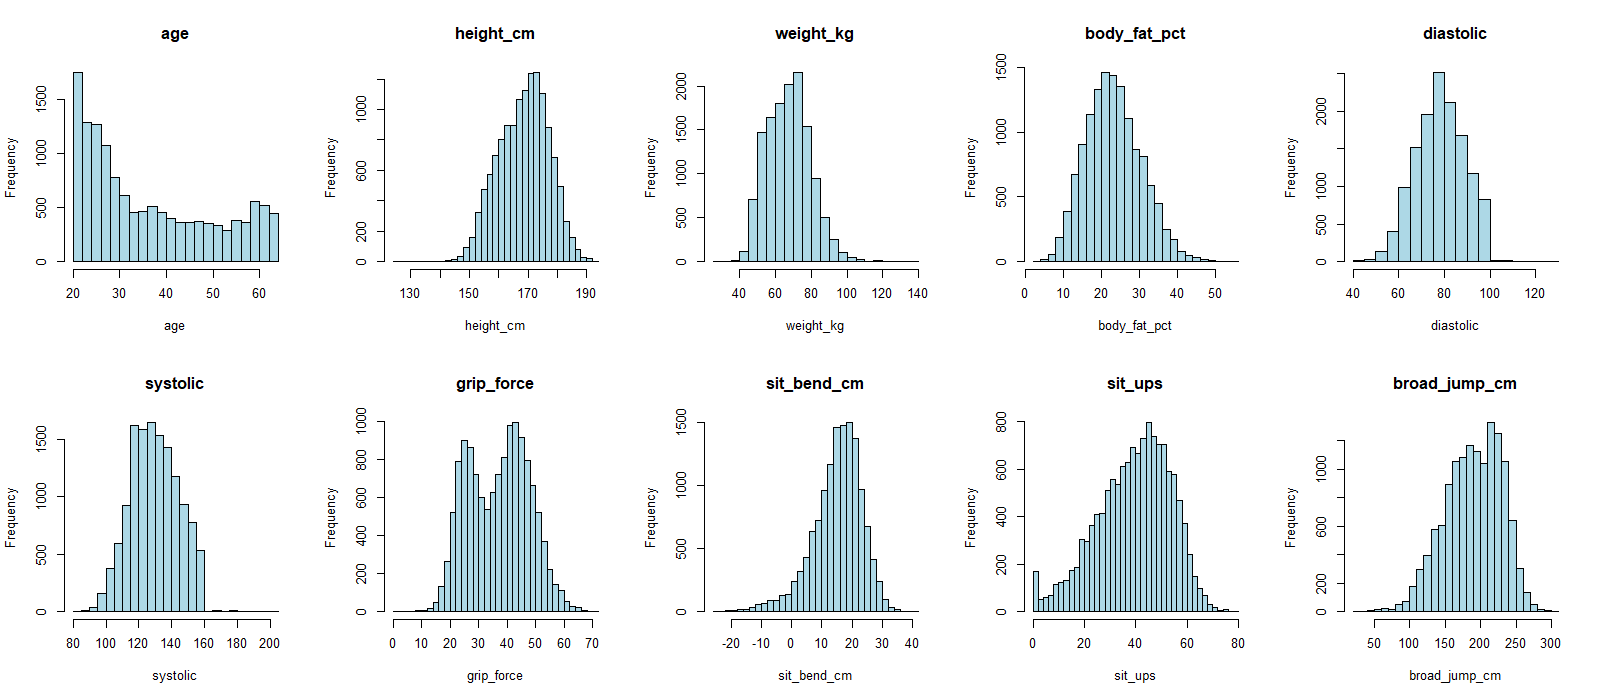
\includegraphics[width=\linewidth]{q1b_histograms}
  \caption{Histograms of the numerical variables (cleaned data).}
  \label{fig:q1b-histograms}
\end{figure}

\begin{figure}[htbp]
  \centering
  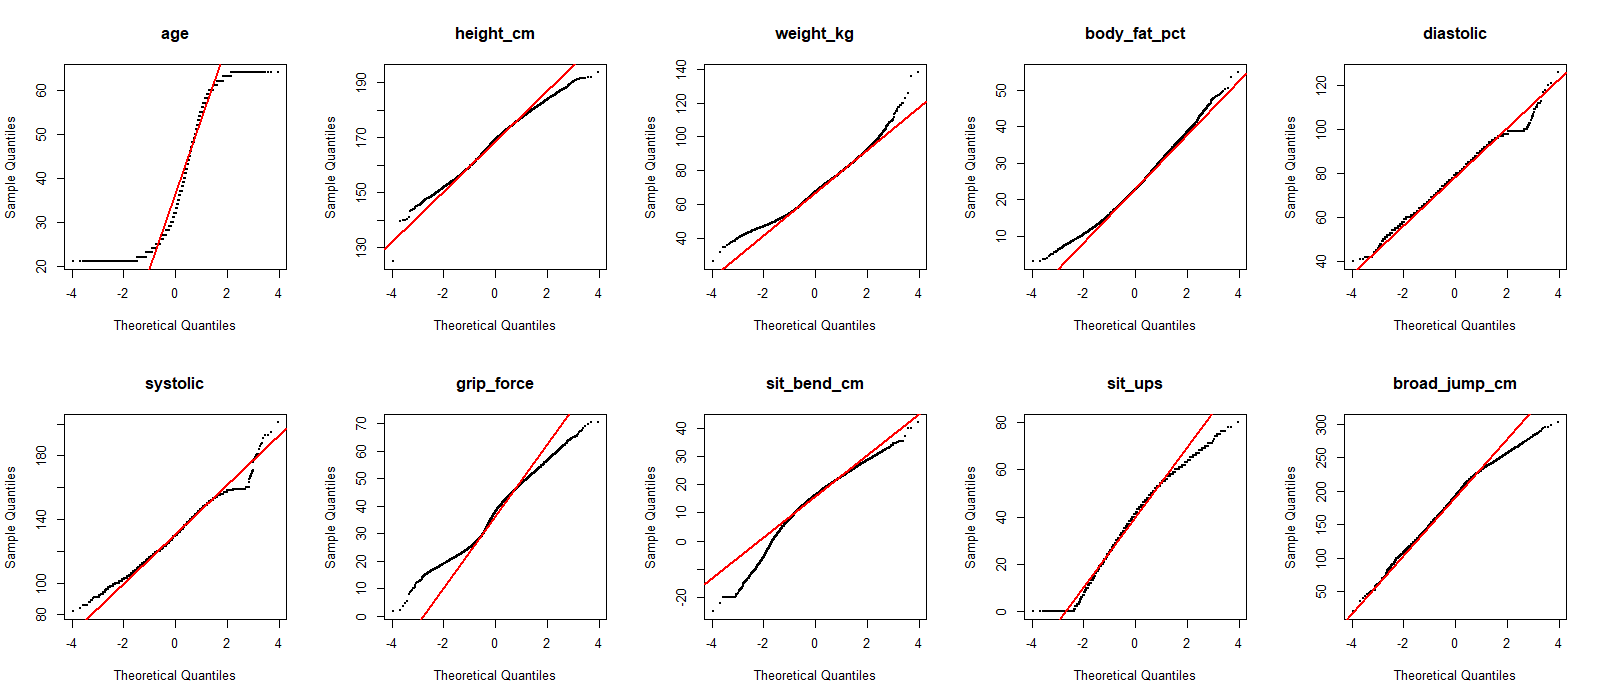
\includegraphics[width=\linewidth]{q1b_qqplots}
  \caption{Normal Q-Q plots of the numerical variables (cleaned data; red line: normal distribution).}
  \label{fig:q1b-qqplots}
\end{figure}

\begin{figure}[htbp]
  \centering
  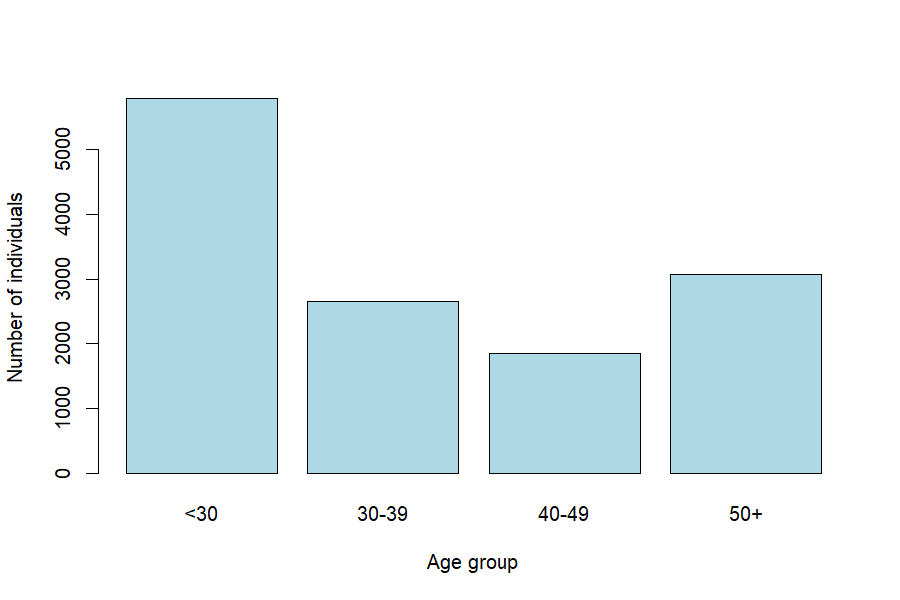
\includegraphics[width=0.6\linewidth]{q1e_age_groups}
  \caption{Number of individuals in each age group.}
  \label{fig:q1e-age-groups}
\end{figure}

\begin{figure}[htbp]
  \centering
  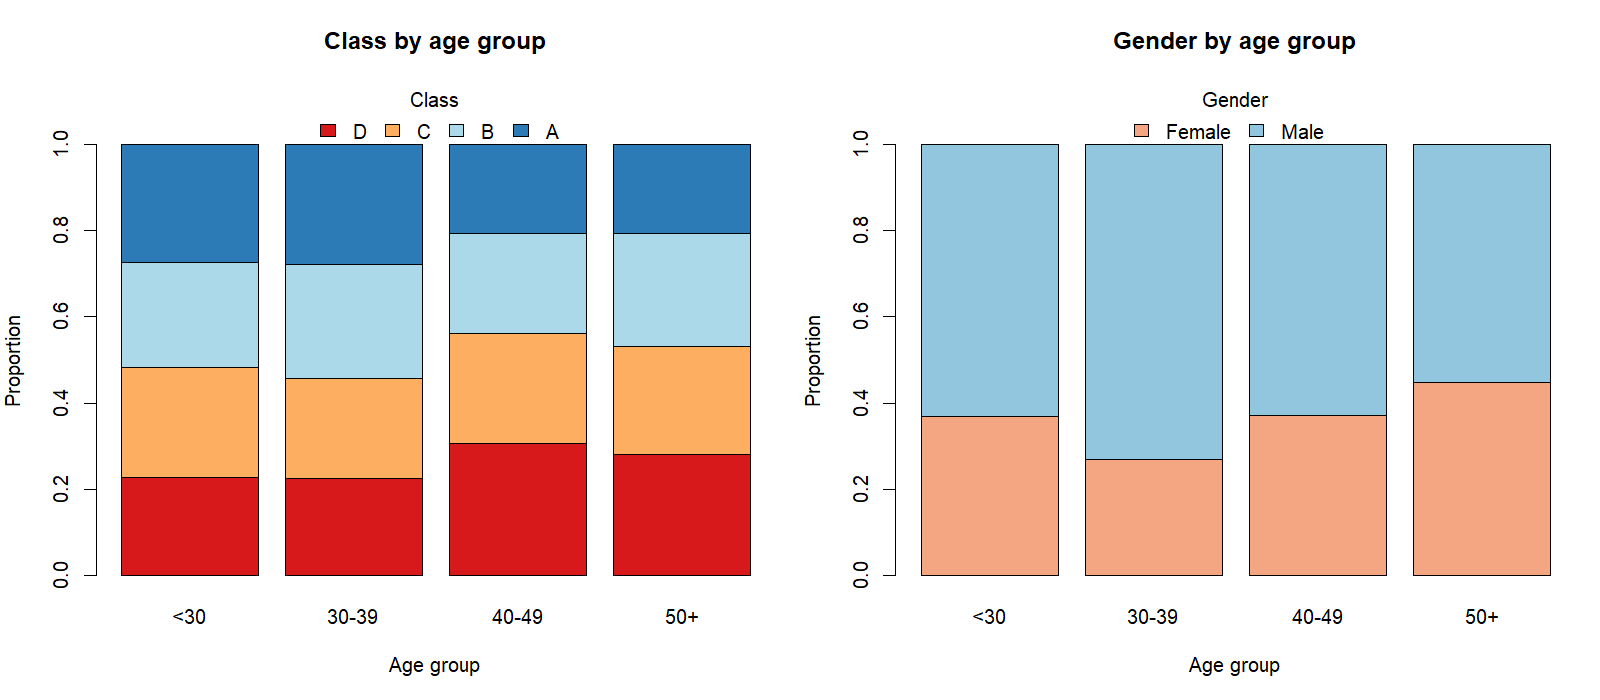
\includegraphics[width=\linewidth]{q1f_proportions}
  \caption{Proportion of each performance class (left) and gender (right) in each age group.}
  \label{fig:q1f-proportions}
\end{figure}

% ============================================================
% APPENDIX C: R CODE AND OUTPUTS
% ============================================================
\clearpage
\section{R Code and Outputs}\label{app:code}

The analysis is done in R, with one script per question in the \texttt{R/} folder of the project: \texttt{R/Q1.R}, \texttt{R/Q2.R} and \texttt{R/Q3.R}, with one section per part of the question.

Each script writes three kinds of output: the tables as CSV files (Appendix~\ref{app:tables}), the charts as PNG files (Appendix~\ref{app:figures}), and its full console output in a log, \texttt{R/logs/<script>.log}.



% ---------- References (refs.bib), after all the figures ----------
\clearpage
\bibliography{refs}

\end{document}
